
\subsection*{1.}

\begin{center}
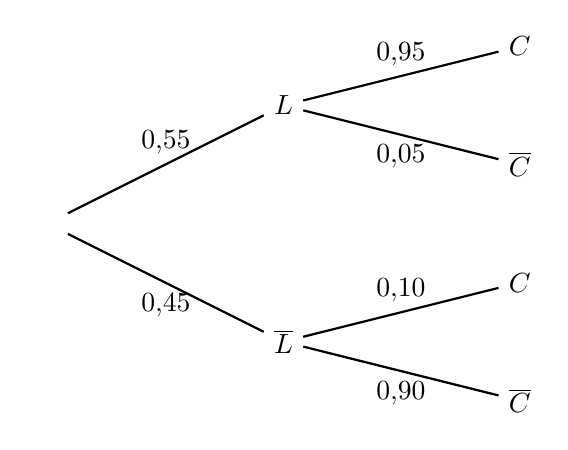
\begin{tikzpicture}[thick, scale=1.5]
\node (P_-1_0) at (-2,-1.5) {$\phantom{A}$};
\node (P_0_0) at (0,-0.5) {$L$};
\draw (P_-1_0) -- (P_0_0) node[midway, above] {$0{,}55$};
\node (P_1_0) at (2,-0) {$C$};
\draw (P_0_0) -- (P_1_0) node[midway, above] {$0{,}95$};
\node (P_1_1) at (2,-1) {$\overline{C}$};
\draw (P_0_0) -- (P_1_1) node[midway, below] {$0{,}05$};
\node (P_0_2) at (0,-2.5) {$\overline{L}$};
\draw (P_-1_0) -- (P_0_2) node[midway, below] {$0{,}45$};
\node (P_1_2) at (2,-2) {$C$};
\draw (P_0_2) -- (P_1_2) node[midway, above] {$0{,}10$};
\node (P_1_3) at (2,-3) {$\overline{C}$};
\draw (P_0_2) -- (P_1_3) node[midway, below] {$0{,}90$};
\end{tikzpicture}
\end{center}

\subsection*{2.}

\(p(L \cap C) = p(L) \times p_L(C) = 0{,}55 \times 0{,}95 = 0{,}5225\).

\subsection*{3.}

D'après la loi des probabilités totales :
\begin{align*}
p(C) &= p(L \cap C) + p(\overline{L} \cap C) \\
&= 0{,}5225 + 0{,}45 \times 0{,}10 \\
&= 0{,}5225 + 0{,}045 \\
&= 0{,}5675.
\end{align*}

\subsection*{4.}

On a :
\[
p_C(L) = \dfrac{p(C \cap L)}{p(C)} = \dfrac{p(L \cap C)}{p(C)} = \dfrac{0{,}5225}{0{,}5675} \approx 0{,}92070,
\]
soit \(0{,}9207\) à \(10^{-4}\) près.

\subsection*{5.}

On a :
\[
p(L) \times p(C) = 0{,}55 \times 0{,}5675 = 0{,}312125 \quad \text{et} \quad p(L \cap C) = 0{,}5225.
\]
\( p(L) \times p(C) \neq p(L \cap C) \) : les événements ne sont pas indépendants.

